\documentclass[12pt,a4paper]{article}

\usepackage[utf8]{inputenc}
\usepackage{amsmath}
\usepackage{amsfonts}
\usepackage{amssymb}
\usepackage[oldstyle, proportional]{libertine}
\usepackage{tabto}
\usepackage{graphicx}
\usepackage{xcolor}
\usepackage{microtype}
\usepackage[colorlinks]{hyperref}
	\hypersetup{
    colorlinks,
    linkcolor={red!50!black},
    citecolor={blue!60!black},
    urlcolor={blue!40!black}
	}
\usepackage[super]{nth}
\usepackage{titlesec}
	\titleformat{\section}{\normalfont\Large\itshape}{\thesection}{0em}{}
	\titleformat{\subsection}{\normalfont\normalsize\bfseries}{\thesubsection}{1em}{}
	%\titlespacing*{\subsection}{0pt}{10pt}{5pt}
\usepackage{enumitem}
	\newlist{collections}{description}{1}
	\setlist[collections]{
		font=\bfseries\normalcolor\ttfamily, 
		before*={\normalfont},  
		topsep=0pt,
		partopsep=0pt,
		parsep=0pt,
		itemsep=0pt
		}
\usepackage{savetrees}
\usepackage{courier}

\begin{document}

\vspace*{-2cm}
\begin{center}
	{\LARGE M. Andrew Jansen, Ph.D.}\\
	\medskip
	{\Large Curriculum Vit\ae}\\
	Updated:~\textit{\today}
\end{center}

\section*{Personal Information}
	\begin{description}		
		\item [Address] \tabto*{2cm} Beltsville Agricultural Research Center, Bldg. 012, Room 1-8 \\
		\tabto*{2cm} 10300 Baltimore Avenue, Beltsville, MD 20705-2325
		\item [Phone] \tabto*{2cm} (301) 504-6649
		\item [E-mail] \tabto*{2cm} \href{mailto:andrew.jansen@usda.gov}{andrew.jansen@usda.gov}
		\item [Website] \tabto*{2cm} \href{https://www.ars.usda.gov/northeast-area/beltsville-md-barc/beltsville-agricultural-research-center/systematic-entomology-laboratory/docs/electron-and-confocal-microscope-unit/}{Electron \& Confocal Microscopy Unit}
		\item [GitHub] \tabto*{2cm} \href{https://github.com/entojansen}{github.com/entojansen}
	\end{description}

\section*{Current Employment}
\subsection*{2022 - Present}
\begin{description}
	\item [Employer] \tabto*{2cm} United States Department of Agriculture
	\item \tabto*{2cm} Agricultural Research Service (Northeast Area)
	\smallskip
	\item [Position] \tabto*{2cm} Research Entomologist -- Systematic Entomology Laboratory
	\item \tabto*{2cm} Director -- Electron and Confocal Microscopy Unit
\end{description}

\section*{Research Interests}
	Microscopy and bioimaging;
	structural adaptation and morphological optimization;
	mechanical behavior of biomaterials;
	insect evolution and biomechanics;
	biomimetic design of robotic systems and materials.

\section*{Education}
	\begin{description}
		\item [2020 - 2022] Postdoctoral Fellowship, University of Bonn. Advisor: Dr. Alexander Blanke
		\\ \href{https://cordis.europa.eu/project/id/754290}{ERC Starting Grant (Recipient: Alexander Blanke, Grant agreement ID: 754290) ``\textbf{MECH-EVO-INSECT}''}
		\item [2014 - 2019] Ph.D., Arizona State University, Evolutionary Biology. Advisor: Dr. Nico Franz
		\\ \href{https://repository.asu.edu/items/53836}{``Evolutionary Biomechanics of the Rostrum of \textit{Curculio} Linnaeus, 1758
		(Coleoptera: Curculionid\ae)''}
		\item [2012 - 2014] M.Sc., Arizona State University, Biology.
		\\ \href{https://repository.asu.edu/items/25115}{``A Phylogenetic Revision of \textit{Minyomerus} Horn, 1876 and \textit{Piscatopus} Sleeper, 1960
		(Curculionid\ae: Entimin\ae: Tanymecini: Tanymecina)''}
		\item [2007 - 2011] B.S., University of Florida, Entomology and Nematology.
	\end{description}

\section*{Peer Reviewed Publications}
	\begin{description}
		\itemsep 0.5em
		
		\item Valente, M., Streett, H., Turner, R., O’Brien, C., Fournet, V., \textbf{Jansen, M.A.}, Dubey, J., Rosenthal, B., Jenkins, M., \& A. Khan. 2024. Morphological and autofluorescence assessment of oocysts differentiate live from dead coccidian parasites. \textit{International Journal for Parasitology}. \textit{In ARS Internal Review}. [ARS 115 Log no. 415935]
		
		\item Jenkins, M., Parker, C., \textbf{Jansen, M.A.}, Papadopoulos, M., \& M. Tucker. 2024. Molecular Characterization of cDNA Coding for 33.5 kDa and 41 kDa Oocyst and Sporocyst Proteins that are Differentially Regulated in Different Strains of Eimeria maxima. \textit{Frontiers in Veterinary Science: Section Parasitology}. \href{https://doi.org/10.3389/fvets.2024.1445646}{11 - 2024}
		
		\item Franco Mel\'{e}ndez, K.P., Schuster, L., Donahey, M.C., Kairalla, E., \textbf{Jansen, M.A.}, Reisch, C., \& A.R. Rivers. 2024. MicroMPN: Methods and software for high-throughput screening of microbe suppression in mixed populations. \textit{Microbiology Spectrum.} \href{https://doi.org/10.1128/spectrum.03578-23}{12: e03578-23}
		
		\item Vieira, P., Kantor, M.R., \textbf{Jansen, M.A.}, Handoo, Z.A., \& J.D. Eisenback. 2023. Cellular insights of beech leaf disease reveal abnormal ectopic cell division of symptomatic interveinal leaf areas. \textit{PLOS ONE}. \href{https://doi.org/10.1371/journal.pone.0292588}{0292588}
		
		\item Inaba, J., Kim, B.M., Zhao, Y., \textbf{Jansen, M.A.}, W. Wei. 2023. The endoplasmic reticulum is a key battleground between phytoplasma aggression and host plant defense. \textit{Cells}. \href{https://doi.org/10.3390/cells12162110}{12(16): 2110}
		
		\item Dougherty, L., Borejsza-Wysocka, E., Miaule, A., Wang, P., Zheng, D., \textbf{Jansen, M.A.}, Brown, S., Pineros,~M., Dardick, C., \& K. Xu. 2023. A single amino acid substitution in MdLAZY1A dominantly impairs shoot gravitropism in \textit{Malus}. \textit{Plant Physiology}. \href{https://doi.org/10.1093/plphys/kiad373}{kiad373}
		
		\item \textbf{Jansen, M.A.}, Niverty, S., Chawla, N., \& N.M. Franz. 2021. Reducing the risk of rostral bending failure in \textit{Curculio} Linnaeus, 1758. \textit{Acta Biomaterialia}. \href{https://doi.org/10.1016/j.actbio.2021.03.029}{126: p. 350-371.}
		
		\item \textbf{Jansen, M.A.}, Williams, J., Chawla, N., \& N.M. Franz. 2019. Avoidance of catastrophic structural failure as an evolutionary constraint: Biomechanics of the acorn weevil rostrum. \textit{Advanced Materials}. \href{https://doi.org/10.1002/adma.201903526}{31(41): 1903526.}
		
		\item \textbf{Jansen, M.A.} \& N.M. Franz. 2018. Descriptions of four new species of \textit{Minyomerus} Horn, 1876 (Coleoptera: Curculionid\ae), with notes on their distribution and phylogeny. \textit{PeerJ}. \href{https://peerj.com/articles/5633/}{6: e5633.}
		
		\item \textbf{Jansen, M.A.}, Luck, K., Campbell, J., Amor, H.B., \& D. Aukes. 2017. Bio-inspired robot design considering load-bearing and kinematic ontogeny of Chelonioidea sea turtles. In \textit{Biomimetic and Biohybrid Systems}. \href{http://www.springer.com/us/book/9783319635361}{p. 216-229}
		
		\item Luck, K., \textbf{Jansen, M.A.}, Campbell, J., Aukes, D., \& H.B. Amor. 2017. From the lab to the desert: fast prototyping and learning of robot locomotion. \textit{Proceedings of Robotics: Science and Systems}. \href{http://www.roboticsproceedings.org/rss13/p75.html}{13: p. 75-83}.
		
		\item \textbf{Jansen, M.A.}, Singh, S.S., Chawla, N., \& N.M. Franz. 2016. A multilayer micromechanical model of the cuticle of \textit{Curculio longinasus} Chittenden, 1927 (Coleoptera: Curculionid\ae). \textit{Journal of Structural Biology}. \href{http://www.sciencedirect.com/science/article/pii/S1047847716300922}{195: p. 139-158.}
		
		\item Singh, S.S., \textbf{Jansen, M.A.}, Franz, N.M., \& N. Chawla. 2016. Microstructure and nanoindentation of the rostrum of \textit{Curculio longinasus} Chittenden, 1927 (Coleoptera: Curculionid\ae). \textit{Materials Characterization}. \href{http://www.sciencedirect.com/science/article/pii/S1044580316301619}{118: p. 206-211.}
		
		\item \textbf{Jansen, M.A.} \& S.E. Halbert. 2016. Key to Florida Alydid{\ae} (Hemiptera: Heteroptera) and selected exotic pest species. \textit{Insecta Mundi}. \href{http://journals.fcla.edu/mundi/article/view/87952/84644}{0476: p. 1-14.}
		
		\item \textbf{Jansen, M.A.} \& N.M. Franz. 2015. Phylogenetic revision of \textit{Minyomerus} Horn, 1876 sec. Jansen \& Franz, 2015 (Coleoptera, Curculionid\ae) using taxonomic concept annotations and alignments. \textit{ZooKeys}. \href{http://zookeys.pensoft.net/articles.php?id=6001}{528: p. 1-133.}
	\end{description}
	
	\subsection*{Featured Media}
	\begin{description}
		\itemsep0.5em
		\item Tuir\'{a}n, R. 2023. ``This weevil has puppet vibes but drills like a power tool''. \textit{KQED, Deep Look}. Electronic version of the Japanese Business Daily. \href{https://www.kqed.org/science/1985068/this-weevil-has-puppet-vibes-but-drills-like-a-power-tool}{14 November}.
		\item Shimonoya, R. 2020. ``The strongest bug, uncrushed by a car, reveals its secret of robustness''. \textit{Nikkei, Technology Column}. Electronic version of the Japanese Business Daily. \href{https://www.nikkei.com/article/DGXMZO66746060X21C20A1MY1000/}{28 November}.
		\item Clement, M. 2019. ``Weevil genius: Insect inspires stronger, more flexible materials''. \textit{ASU Now}. \href{https://asunow.asu.edu/20191010-discoveries-asu-engineering-weevil-inspires-stronger-flexible-materials}{10 October}.
		
	\end{description}

	\subsection*{Manuscripts in Preparation}
		\begin{description}
			\itemsep0.5em
			\item \textbf{Jansen, M.A.}, Fife, A., Hanzlik, M., \& F. Bai. Direct imaging of live plant tissue using VP-SEM through vascular support by stem encapsulation. \textit{In Prep}.
			\item \textbf{Jansen, M.A.} Descriptions and distributions of four new species of \textit{Minyomerus} Horn, 1876 (Coleoptera: Curculionid\ae). \textit{In Prep}.
			\item \textbf{Jansen, M.A.} \& A. Blanke. Set-theoretic classification of unidirectional plies in the cuticle of Polyneoptera. \textit{In Prep}.
		\end{description}
	
	\subsection*{Protocols}
	\begin{description}
		\itemsep0.5em
		\item Franco Mel\'{e}ndez, K.P., Schuster, L., Donahey, M.C., Kairalla, E., \textbf{Jansen, M.A.}, Reisch, C., \& A.R. Rivers. 2023. MicroMPN: Software and methods for high-throughput screening of microbe suppression in mixed populations. protocol published via \href{dx.doi.org/10.17504/protocols.io.81wgbymenvpk/v1}{protocols.io}
		\item Franco Mel\'{e}ndez, K.P., Schuster, L., Donahey, M.C., Kairalla, E., \textbf{Jansen, M.A.}, Reisch, C., \& A.R. Rivers. 2023. Most Probable Number Fluorescence Microplate Assay V.1. protocol published via \href{dx.doi.org/10.17504/protocols.io.q26g7yqk1gwz/v1}{protocols.io}
	\end{description}

\section*{Conference Presentations}
	\begin{description}
		\itemsep0.5em
		\item \textbf{Jansen, M.A.}, Luktuke, A., Chawla, N., Labonte, D., \& A. Blanke. 2022. ``Evidence of functionally graded cuticle	in Polyneopteran head capsules''. \textit{\nth{26}~International Congress of Entomology}, Helsinki, FI.
		\item \textbf{Jansen, M.A.}, Luktuke, A., Chawla, N., Labonte, D., \& A. Blanke. 2023. ``Evidence of functionally graded cuticle in Polyneopteran head capsules''. \textit{Annual Meeting of the Entomological Society of America}, Washington, DC.
		\item \textbf{Jansen, M.A.} 2023. ``Insect cuticle is for entomologists, not engineers''. \textit{Monthly Meeting (March) of the Entomological Society of Washington}, Washington, DC.
		\item \textbf{Jansen, M.A.}, Luktuke, A., Chawla, N., Labonte, D., \& A. Blanke. 2022. ``Characterization of insect cuticle: challenges and insights''. \textit{Annual Meeting of the Society for Experimental Biology}, Montpellier, FR.
		\item \textbf{Jansen, M.A.}, Luktuke, A., Chawla, N., Labonte, D., \& A. Blanke. 2022. ``Evidence of functionally graded cuticle	in Polyneopteran head capsules''. \textit{\nth{26}~International Congress of Entomology}, Helsinki, FI.
		\item \textbf{Jansen, M.A.}, Luktuke, A., Chawla, N., Labonte, D., \& A. Blanke. 2022. ``Evidence of functionally graded cuticle	in Polyneopteran head capsules''. \textit{\nth{5}~International Congress of Invertebrate Morphology}, Vienna, AT.
		\item \textbf{Jansen, M.A.}, \& N.M. Franz. 2018. ``Comparative bending mechanics and morphology of the snout in \textit{Curculio} Linnaeus 1756''. \textit{Annual Meeting of the Entomological Society of America}, Vancouver, BC.
		\item \textbf{Jansen, M.A.}, Chawla, N., \& N.M. Franz. 2017. ``Fracture mechanics and evolution of resilient cuticle in the rostrum of \textit{Curculio} Linnaeus, 1758''. \textit{Annual Meeting of the Entomological Society of America}, Denver, CO.
		\item \textbf{Jansen, M.A.} \& N.M. Franz. 2017. ``Evolutionary mechanics of the rostrum in \textit{Curculio} Linnaeus, 1758''. \textit{Annual Meeting of the Willi Hennig Society}, St. Petersburg, FL.
		\item \textbf{Jansen, M.A.}, Luck, K., Campbell, J., Amor, H.B., \& D. Aukes. 2017. ``Bio-inspired robot design considering load-bearing and kinematic ontogeny of Chelonioidea sea turtles''. \textit{Living Machines}, Stanford, CA.
		\item Luck, K., \textbf{Jansen, M.A.}, Campbell, J., Aukes, D., \& H.B. Amor. 2017. ``From the lab to the desert: fast prototyping and learning of robot locomotion''. \textit{Robotics: Science and Systems}, Cambridge, MA.
		\item \textbf{Jansen, M.A.} \& N.M. Franz. 2016. ``Why the long face? Insights into the mechanical behavior of the rostrum in the genus \textit{Curculio} Linnaeus, 1758''. International Congress of Entomology, Orlando, FL.
		\item \textbf{Jansen, M.A.}, Singh, S.S., Chawla, N., \& N.M. Franz. 2015. ``Mechanical Behavior of the Rostrum of \textit{Curculio} Linnaeus, 1758 (Coleoptera: Curculionid\ae)''. Annual Meeting of the Entomological Society of America, Minneapolis, MN.
		\item \textbf{Jansen, M.A.} \& N.M. Franz. 2014. ``A phylogenetic revision of \textit{Minyomerus} Horn, 1876, and \textit{Piscatopus} Sleeper, 1960 (Coleoptera: Curculionid\ae: Entimin\ae: Tanymecini)''. Annual Meeting of the Entomological Society of America Pacific Branch, Tucson, AZ.
		\item \textbf{Jansen, M.A.} \& N.M. Franz. 2013. ``A phylogenetic revision of \textit{Minyomerus} Horn, 1876, and \textit{Piscatopus} Sleeper, 1960 (Coleoptera: Curculionid\ae: Entimin\ae: Tanymecini)''. Annual Meeting of the Entomological Society of America, Austin, TX.
		\item \textbf{Jansen, M.A.} \& N.M. Franz. 2013. ``A phylogenetic revision of \textit{Minyomerus} Horn, 1876, and \textit{Piscatopus} Sleeper, 1960 (Coleoptera: Curculionid\ae)''. 12th Biennial Conference of Science and Management on the Colorado Plateau, Flagstaff, AZ.
	\end{description}

\section*{Awards and Fellowships}
	\begin{description}
		\item [2024] \$588,002.00 - USDA-ARS, NP303: Plant Diseases, Project \textnumero: 8042-22000-305-00D, ``Advanced Microscopy for Fundamental Research of Agricultural Pests and Pathogens'', Lead Scientist
		\item [2023] \$71,555.55 - USDA-NIFA, Project \textnumero: 8042-22000-313-002R, ``Developing Sustainable Rose Landscapes via RRD Assessments and Breeding RRD Resistant Roses with Stable Blackspot Resistance'', Cooperator
		\item [2019] \$12,000.00 - ASU School of Life Sciences Completion Fellowship
		\item [2018] Awarded honorary 1-year membership - AAAS/Science Excellence in Science Program
		\item [2018] \$400.00 - ASU School of Life Sciences Fall Travel Award
		\item [2018] \$500.00 - ASU Q2 Graduate College Travel Award
		\item [2018] \$12,250.00 - ASU Biomimicry Center Fellowship (Corporate sponsorship by Google, Inc.)
		\item [2017] \$500.00 - The Willi Hennig Society Student Travel Award
		\item [2017] \$400.00 - ASU School of Life Sciences Fall Travel Award
		\item [2017] \$195.00 - ASU Q2 Graduate College Travel Award
		\item [2017] \$6,000.00 - ASU Evolutionary Biology Doctoral Program Summer Fellowship
		\item [2016] \$400.00 - ASU School of Life Sciences Fall Travel Award
	\end{description}

\section*{Products Developed}
	\subsection*{C-Turtle}
		\begin{description}
			\itemsep0em
			\item[Website] \href{https://sites.google.com/view/c-turtle/}{https://sites.google.com/view/c-turtle/}
			\item[Design] \href{https://drive.google.com/file/d/0BxntR7XVPIVqekR3Sjcyd1hkUm8/view}{Version 1.0 Cut-files}
			\item[License] \href{https://creativecommons.org/licenses/by/4.0/}{Attribution 4.0 International} (CC BY 4.0)
		\end{description}

	\subsection*{Patent Applications}
		\begin{description}
			\itemsep0.5em
			\item Aukes, D., Amor, H.B., Luck, K., \textbf{Jansen, M.A.}, \& J. Campbell, \textit{inventors}; Arizona State University, Skysong Innovations, \textit{assignee}. 2018. United States non-provisional patent application for systems and methods for rapid-prototyped robotic devices. \textit{US Patent Application No. 16/215,910}. Filed 11 December 2018.
			
			\item Aukes, D., Amor, H.B., Luck, K., \textbf{Jansen, M.A.}, \& J. Campbell, \textit{inventors}; Arizona State University, Skysong Innovations, \textit{assignee}. 2017. United States provisional patent application for systems and methods for rapid-prototyped robotic devices. \textit{US Patent Application No. 62/597,276}. Filed 11 December 2017.
		\end{description}

	\subsection*{Featured Media}
		\begin{description}
			\itemsep0.15em
			\item Adams, D. 2017. ``An army of these odd-looking robotic 'turtles' might help rid the world of landmines''. \textit{Digital Trends}. \href{https://www.digitaltrends.com/cool-tech/robot-turtles-detect-landmines/}{26 May}.
			\item Ander, J. 2017. ``Landmine-clearing Pi-powered C-Turtle''. \textit{Raspberry Pi Official Blog}. \href{https://www.raspberrypi.org/blog/landmine-c-turtle/}{26 July}.
			\item Coledewey, D. 2017. ``These flat-pack turtlebots will crawl across minefields for safety's sake''. \textit{Tech Crunch}. \href{https://techcrunch.com/2017/05/25/these-flat-pack-turtlebots-will-crawl-across-minefields-for-safetys-sake/}{25 May}.
			\item Crookes, D. 2017. ``C-TURTLE''. \textit{The MagPi Magazine}: Issue 63 \href{https://www.raspberrypi.org/magpi/c-turtle/}{1 November}.
			\item DeLisle, J.J. 2017. ``Raspberry-Pi-powered turtle robot learns to navigate new terrains on its own - From planetary exploration to swarm robotic landmine sensing, C-Turtle's possibilities are endless''. \textit{Electronic Products}. \href{https://www.electronicproducts.com/Robotics/AI/Raspberry_Pi_powered_turtle_robot_learns_to_navigate_new_terrains_on_its_own.aspx}{11 August}.
			\item Fagan, K. 2017. ``The landmine-detecting robot `turtle'". \textit{BBC News}. \href{http://www.bbc.com/news/av/technology-40296297/the-soft-3d-printed-robot-that-could-come-to-the-rescue}{22 July}.
			\item Horsey, J. 2017. ``Raspberry Pi used to create C-Turtle, landmine clearing robot''. \textit{Geeky Gadgets}. \href{https://www.geeky-gadgets.com/landmine-clearing-robot-27-07-2017/}{27 July}.
			\item Kety, S. 2017. ```C-Turtle', the 3D printed robot whose movements are similar to a sea turtle''. \textit{3D Adept News}. \href{https://3dadept.com/c-turtle-the-3d-printed-robot-whose-movements-are-similar-to-a-sea-turtle/}{16 August}.
			\item Koslow, T. 2017. ``Out of the shell - C-Turtle: the paper turtle robot that can detect landmines''. \textit{All3DP}. \href{https://all3dp.com/landmine-detecting-robot-c-turtle/}{20 August}.
			\item Lavars. N. 2017. ``Turtle-bot teaches itself to waddle through the desert''. \textit{New Atlas}. \href{https://newatlas.com/turtle-robot-self-learning-waddle/49738/}{26 May}.
			\item Ludacer, R. 2017. ``Researchers are using robotic sea turtles to find land mines''. \textit{Tech Insider}. \href{https://www.facebook.com/techinsider/videos/787578874773804/}{10 June}.
			\item Ray, A. 2017. ``A new turtle explorer - This \$70 robot that mimics a sea-turtle may eventually reach Mars''. \textit{Quartz}. \href{https://qz.com/1053078/this-70-robot-that-mimics-a-sea-turtle-may-eventually-reach-mars/}{15 August}.
			\item Massaouden, L. 2017. ``C-Turtle, le robot tortue en carton qui doit un jour explorer Mars''. \textit{Mashable avec France 24}. \href{http://mashable.france24.com/videos/20170825-c-turtle-robot-tortue-carton-exploration-mars}{25 August}.
			\item Mathews, L. 2017. ``Robotic Turtles With Raspberry Pi Brains Are Sniffing Out Land Mines''. \textit{Geek.com}. \href{https://www.geek.com/tech/robotic-turtles-with-raspberry-pi-brains-are-sniffing-out-land-mines-1709339/}{27 July}.
			\item Sabin, D. 2017. ``This crawling C-Turtle robot could hunt for landmines''. \textit{Inverse}. \href{https://www.inverse.com/article/32219-cturtle-robot-sea-turtle-mines}{26 May}.
			\item Reynolds, M. 2017. ``Robotic turtles can be used to detect landmines in the desert''. \textit{New Scientist Magazine}: Issue 3127. \href{https://www.newscientist.com/article/mg23431274-200-robotic-turtles-can-be-used-to-detect-landmines-in-the-desert/}{24 May}.
			\item Sant, J.V. 2017. ``ASU Robotics turns to nature for inspiration''. KPHO Broadcasting Corporation: \textit{3TV/CBS5}. \href{http://www.azfamily.com/story/35595946/asu-robotics-turns-to-nature-for-inspiration}{5 June}.
			\item Scott, C. 2017. ``Partially 3D printed C-Turtle robots crawl and adapt in the desert''. \textit{3Dprint.com}. \href{https://3dprint.com/184523/3d-printed-c-turtle-robots/}{17 August}.
			\item Seckel, S. 2017. ``Technology comes from collaboration between computer science, mechanical engineering and biology''. \textit{ASU Now}. \href{https://asunow.asu.edu/20170525-solutions-asu-designed-c-turtle-robot-teaches-itself-get-around}{25 May}.
			\item Seckel, S. 2017. ``ASU-designed C-Turtle robot teaches itself to get around''. \textit{ASU Now}. \href{https://asunow.asu.edu/20170525-solutions-asu-designed-c-turtle-robot-teaches-itself-get-around}{25 May}.
			\item Wehner, M. 2017. ``These robotic turtles could save your life''. \textit{New York Post}. \href{https://nypost.com/2017/05/25/these-robotic-turtles-could-save-your-life/}{25 May}.
			\item Unknown - `Hackster Staff'. 2017. ``Nature-inspired C-Turtle robot waddles the desert with ease''. \textit{Hackster}. \href{https://blog.hackster.io/nature-inspired-c-turtle-robot-waddles-the-desert-with-ease-3061cbc19b36}{26 May}.
			\item Unknown - `Gadget Junkie'. 2017. ``C-Turtle: cardboard turtle robot with Raspberry Pi''. \textit{gadgetify}. \href{http://www.gadgetify.com/c-turtle-cardboard-turtle-robot/}{27 July}.
			\item Unknown - `Robot Man'. 2017. ``C-Turtle cardboard robot turtle learns to navigate different terrains''. \textit{Robotic Gizmos}. \href{http://www.roboticgizmos.com/c-turtle-robot-turtle/}{27 July}.
		\end{description}

\section*{Design and Prototyping Services}
	\subsection*{Western Entomological Supply (Co-founder)}
		\href{https://github.com/western-entomological}{github.com/western-entomological}
		\begin{description}
			\item [2017 - 2019] Design and production of insect mounting points for entomological collections (Universal Laser Cutter VLS 6.60)
			\item [2017 - 2019] Design and production of curation equipment for insect specimens (MakerBot Replicator 2x)
			\item [2018] Production of cassette cartridge spacer and brackets prototypes for TechShot (MakerBot Replicator 2x)
		\end{description}
	
\section*{Programming Languages and Software}
	\subsection*{Languages}
		\begin{description}
			\item Most proficient with Python, R, and \LaTeX
			\item Intermediate experience with Bash, MATLAB
			\item Dabbled in Abaqus Script, HTML, XML, Java, BASIC, Visual Basic, JavaScript, Git
			\item Currently training in C++17/20
		\end{description}
		
	\subsection*{Software}
		\begin{description}
			\item Most proficient with Zeiss Zen Blue, Solidworks, Abaqus/CAE
			\item Intermediate experience with COMSOL, ImageJ, GraphPad Prism
			\item Dabbled in PrusaSlicer, Amira, Adobe Photoshop, Adobe Illustrator
		\end{description}


\section*{Society Memberships}
	\begin{description}
		\item [2024] Maryland Entomological Society
		\item [2022 - 2024]	Entomological Society of Washington (President-Elect, 2024)
		\item [2013 - 2024] Entomological Society of America
		\item [2013 - 2019] Coleopterists Society
	\end{description}

\section*{Academic Service}
	\subsection*{Manuscript Reviewer}
		\begin{description}
			\item Proceedings of the Entomological Society of Washington
			\item Acta Biomaterialia
			\item The Coleopterists Bulletin
			\item Coleopterists Society Monographs (Patricia Vaurie Series)
			\item The Pan-Pacific Entomologist 
			\item Zootaxa
		\end{description}

	\subsection*{Book Chapter Reviews}
		\begin{description}
			\item ``Weevils (Coleoptera: Dryophthorid\ae, Brachycerid\ae, Erirhinid\ae, Curculionid\ae) of the Prairie Ecozone in Canada''.
					Robert S. Anderson, Patrice Bouchard, \& Hume Douglas.
					In Volume 4 of \textit{Arthropods of Canadian Grasslands}.
		\end{description}

	\subsection*{Community Outreach}
		\begin{description}
			\item [2025] SWRS - Weevil Course 2025
			\item [2024] ESW - Annual Banquet of Entomological Society of Washington
			\item [2024] ECMU - CRAFT Scholars Tour
			\item [2024] ECMU - Office of National Programs Tour
			\item [2023] ECMU - CRAFT Scholars Tour
			\item [2023] ESA - Tour of Beltsville Area Facilities
			\item [2023] ECMU - Microscopy Open House
			\item [2013 - 2018] ASU - SoLS Night of the Open Door
			\item [2013 - 2016] ASU - IAFSE Engineering Open House
			\item [2014 - 2015] ASU - SoLS Graduate Partners in Science Education
			\item [2014] SWRS - Weevil Course 2014
		\end{description}
		
	\subsection*{Insect Identification and Expeditionary Services}
		\begin{description}
			\item [2019] Greater Good, Madrean Discovery Expedition - Sierra Chivato, SO, M\'{e}xico
			\item [2017 - 2018] US Department of Agriculture - Tempe, AZ, USA
			\item [2017] Greater Good, Madrean Discovery Expedition - Caj\'{o}n Bonito, SO, M\'{e}xico
			\item [2014] Madrean Discovery Expedition - Patagonia, AZ, USA
			\item [2013] Madrean Discovery Expedition - Sierra la P\'{u}rica, SO, M\'{e}xico
			\item [2013] US National Park Service, BioBlitz - Joshua Tree National Park, CA, USA
			\item [2012] Madrean Discovery Expedition - Sierra Aconchi, SO, M\'{e}xico
		\end{description}

\section*{Teaching Appointments}
	\begin{tabbing}
		\hspace{2cm}\=\hspace{6.5cm}\=\hspace{4cm}\=\kill
		\textbf{Course} \> \textbf{Subject} \> \textbf{Semester} \> \textbf{Position}\\
		BIO 201 \> Human Anatomy and Physiology \> Fall - 2019 \> Instructor \\
		BIO 386 \> Entomology \> Fall - 2018 \> Instructor \\ 
		BIO 201 \> Human Anatomy and Physiology \> Spring - 2017 \> Teaching Assistant \\
		BIO 281 \> Biology (\nth{1}~~Semester for Majors) \> Fall - 2016 \> Teaching Assistant \\
		BIO 182 \> Biology (\nth{2}~Semester) \> Summer - 2016 \> Teaching Assistant \\
		BIO 181 \> Biology (\nth{1}~Semester) \> Spring - 2016 \> Teaching Assistant \\
		BIO 282 \> Biology (\nth{2}~Semester for Majors) \> Spring 2014 \> Teaching Assistant \\
		BIO 386 \> Entomology \> Fall - 2013, 2014, 2015 \> Teaching Assistant
	\end{tabbing} 

\section*{Field and Museum Work}
	\subsection*{Field Work}
		\begin{description}
			\item [United States] \tabto*{3cm} AZ, CA, CO, DC, FL, GA, ID, MD, NM, NV, PR, SC, TX, UT, VA (2010 - 2024)
			\item [Japan] \tabto*{3cm} JP-01, JP-13, JP-26 (2024)
			\item [Germany] \tabto*{3cm} NRW (2020 - 2022)
			\item [Mexico] \tabto*{3cm} SO (2012, 2013, 2017, 2019)
			\item [Guatemala] \tabto*{3cm} AV, BV, CM, CQ, ES, GU, HU, IZ, JA, PR, QC, QZ, SA, SO, SR, SU, TO, ZA (2014)
		\end{description}

	\subsection*{Collections Visited}
		\begin{collections}
			\item [ASUT] USA, Arizona, Tempe, Arizona State University, Hasbrouck Insect Collection
			\item [BYUC] USA, Utah, Provo, Brigham Young University, Monte L. Bean Life Science Museum
			\item [CASC] USA, California, San Francisco, California Academy of Sciences
			\item [CSCA] USA, California, Sacramento, California State Collection of Arthropods
			\item [CSDS] USA, California, Baker, Desert Studies Center
			\item [CSUC] USA, Colorado, Fort Collins, Colorado State University
			\item [CWOB] USA, Arizona, Green Valley, Charles W. O'Brien Collection
			\item [EIHU] Japan, Hokkaido, Sapporo, Hokkaido University
			\item [EMEC] USA, California, Berkeley, University of California, Essig Museum of Entomology
			\item [FSCA] USA, Florida, Gainesville, Division of Plant Industry, Florida State Collection of Arthropods
			\item [FSMC] USA, Florida, Gainesville, University of Florida, Florida Museum of Natural History
			\item [LBOB] USA, Arizona, Green Valley, Lois B. O'Brien Collection
			\item [MGCL] USA, Florida, Gainesville, University of Florida, McGuire Center for Lepidoptera and Biodiversity
			\item [NAUF] USA, Arizona, Flagstaff, Northern Arizona University
			\item [NMNH] USA, Washington, D.C., Smithsonian Institute, National Museum of Natural History
			\item [NMSU] USA, New Mexico, Las Cruces, New Mexico State University, Museum of Southwestern Biology
			\item [NVDA] USA, Nevada, Reno, Nevada State Department of Agriculture
			\item [RLAC] USA, California, El Dorado Hills, Rolf L. Aalbu Collection
			\item [SMFD] Germany, Hessen, Frankfurt-am-Main, Forschungsinstitut und Naturmuseum Senckenberg
			\item [SWRS] USA, Arizona, Portal, Southwestern Research Station
			\item [TAMU] USA, Texas, College Station, Texas Agricultural and Mechanical University
			\item [TTUZ] USA, Texas, Lubbock, Texas Tech University
			\item [UAIC] USA, Arizona, Tucson, University of Arizona
			\item [UCDC] USA, California, Davis, University of California, R.M. Bohart Museum of Entomology
			\item [UCRC] USA, California, Riverside, University of California, Entomology Research Museum
			\item [UNMC] USA, New Mexico, Albuquerque, University of New Mexico
			\item [UMNH] USA, Utah, Salt Lake City, University of Utah, Utah Museum of Natural History
			\item [UVGC] Guatemala, Guatemala City, Universidad del Valle de Guatemala, Colleci\'{o}n de Artr\'{o}podos
			\item [ZMHB] Germany, Berlin, Museum f\"{u}r Naturkunde der Humboldt Universit\"{a}t zu Berlin
		\end{collections}

\section*{Employment History}
	\begin{description}
		\item [2021] Postdoctoral Researcher - University of Bonn
		\item [2020] Postdoctoral Researcher - University of Cologne
		\item [2019] Adjunct Instructor - Mesa Community College
		\item [2019] Research Consultant - The Biomimicry Center, Arizona State University
		\item [2012] Museum Technician - Florida State Collection of Arthropods \& McGuire Center for Lepidoptera
		\item [2011] Research Technician - Honeybee Research and Extension Laboratory, University of Florida
		\item [2011] Research Assistant - Division of Insect Behavior, USDA-ARS, Gainesville, FL
		\item [2009 - 2011] Senior Counsellor - Center for Precollegiate Education and Training, University of Florida
	\end{description}

\vspace{1cm}

\noindent\large{\textbf{Professional references available upon request.}}

\vspace*{1cm}
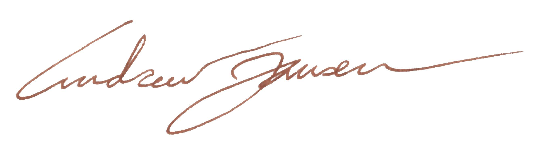
\includegraphics[scale=1]{signature.pdf}\\

\end{document}